\renewcommand\drawNodes[2]{
  % #1 (str): namespace
  % #2 (list[list[str]]): list of labels to print in the node of each neuron
  \foreach \neurons [count=\lyrIdx] in #2 {
    \StrCount{\neurons}{,}[\lyrLength] % use xstring package to save each layer size into \lyrLength macro

    \ifthenelse{\equal{#1}{encoder}}{
        \ifnumequal{\lyrIdx}{1}
        {% True case
        \foreach \n [count=\nIdx] in \neurons
            \node[neuron,fill=green,fill opacity=0.2] (#1-\lyrIdx-\nIdx) at (0.7*\lyrIdx, \lyrLength/3.6-0.5*\nIdx) {\n};
        }
        {% False case
        \foreach \n [count=\nIdx] in \neurons
            \node[neuron] (#1-\lyrIdx-\nIdx) at (0.7*\lyrIdx, \lyrLength/3.6-0.5*\nIdx) {\n};
        }
    }{
        \ifnumequal{\lyrIdx}{2}
        {% True case
        \foreach \n [count=\nIdx] in \neurons
            \node[neuron,fill=green,fill opacity=0.2] (#1-\lyrIdx-\nIdx) at (0.7*\lyrIdx, \lyrLength/3.6-0.5*\nIdx) {\n};
        }
        {% False case
        \foreach \n [count=\nIdx] in \neurons
            \node[neuron] (#1-\lyrIdx-\nIdx) at (0.7*\lyrIdx, \lyrLength/3.6-0.5*\nIdx) {\n};
        }
    }
  }
}

\renewcommand\denselyConnectNodes[2]{
  % #1 (str): namespace
  % #2 (list[int]): number of nodes in each layer
  \foreach \n [count=\lyrIdx, remember=\lyrIdx as \previdx, remember=\n as \prevn] in #2 {
    \foreach \y in {1,...,\n} {
      \ifnum \lyrIdx > 1
        \foreach \x in {1,...,\prevn}
          \draw[-] (#1-\previdx-\x) -- (#1-\lyrIdx-\y);
      \fi
    }
  }
}

\begin{tikzpicture}[
    shorten >=1pt, shorten <=1pt,
    neuron/.style={circle, draw, minimum size=2ex, thick},
    legend/.style={font=\large\bfseries},
  ]

  % encoder
  \drawNodes{encoder}{{{,,,,,}, {,,}}}
  \denselyConnectNodes{encoder}{{6, 3}}

  % decoder
  \begin{scope}[xshift=3.7cm]
    \drawNodes{decoder}{{{,,}, {,,,}}}
    \denselyConnectNodes{decoder}{{3, 4}}
  \end{scope}
  
  \node[inner sep=0pt,left of=encoder-1-1,xshift=-0.5cm,yshift=-0.2cm] (input) {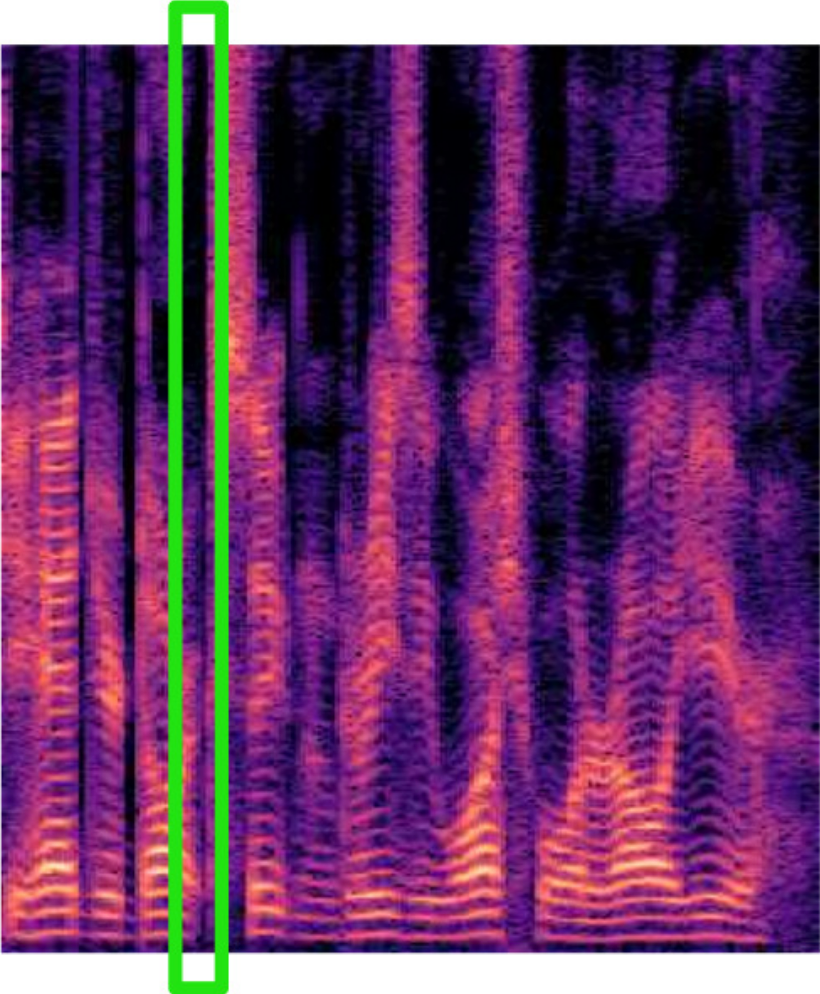
\includegraphics[width=.25\textwidth]{tikz/spectrogram}};
  \node[inner sep=0pt,left of=encoder-1-1,xshift=-0.5cm,yshift=-2.4cm] (input2) {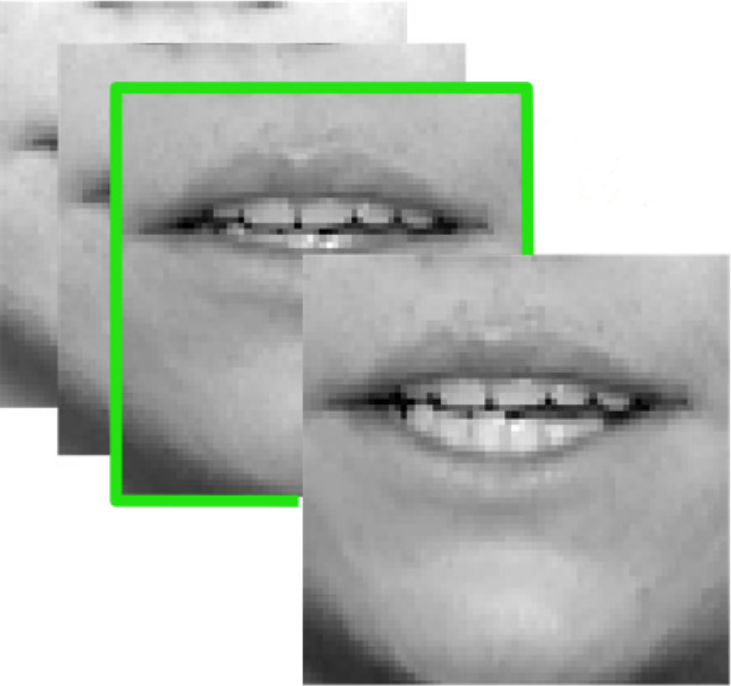
\includegraphics[width=.25\textwidth]{tikz/lips}};
  \node[inner sep=0pt,right of=decoder-2-1,xshift=0.5cm,yshift=-0.8cm] (output) {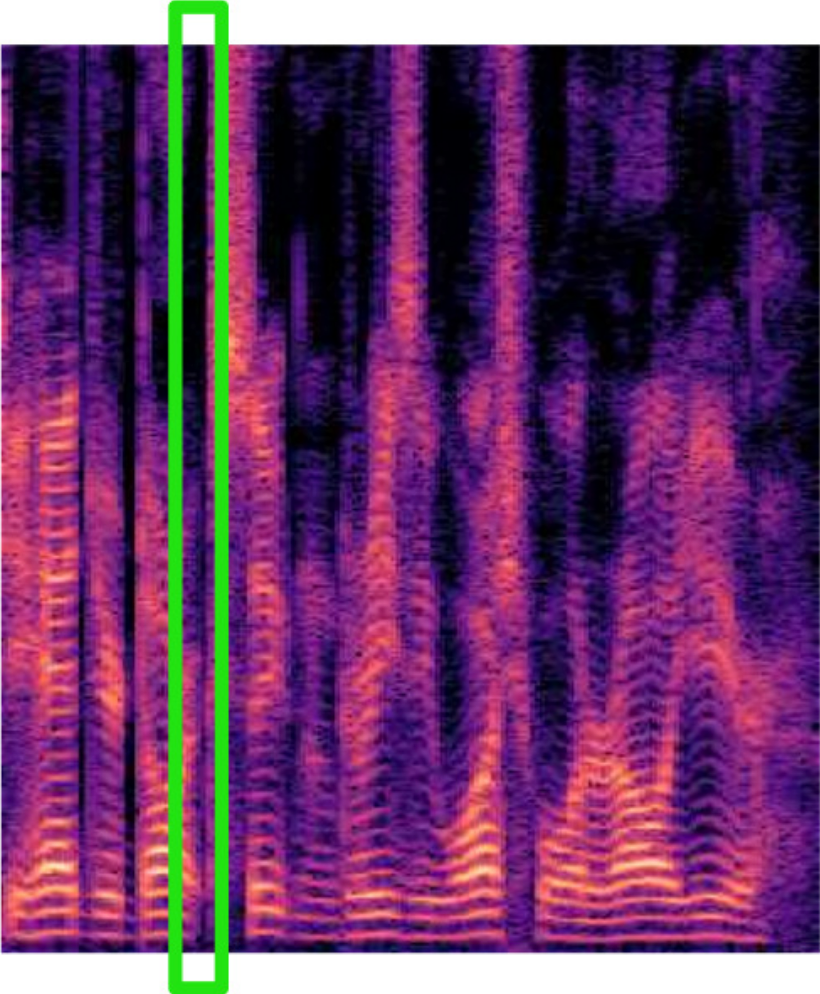
\includegraphics[width=.25\textwidth]{tikz/spectrogram}};
  
  % mu, sigma, sample nodes, conditioning
  \foreach \idx in {1,...,3} {
      \coordinate[neuron, right=2 of encoder-2-2, xshift=-1.4cm, yshift=0.5*\idx cm-0.15cm, fill=red, fill opacity=0.2] (mu-\idx);
      \coordinate[neuron, right=2 of encoder-2-2, xshift=-1.4cm, yshift=-0.5*\idx cm+0.15cm, fill=red, fill opacity=0.2] (sigma-\idx);
      \coordinate[neuron, right=4 of encoder-2-2, xshift=-2.2cm, yshift=0.5*\idx cm-.15cm, fill=red, fill opacity=0.2] (sample-\idx);
      \coordinate[neuron, right=4 of encoder-2-2, xshift=-2.2cm, yshift=0.5*\idx cm-1.85cm, fill=green, fill opacity=0.2] (cond-\idx);
    }
    
  \node[inner sep=0pt,below of=cond-1,xshift=0.2cm,yshift=0.2cm] (cond) {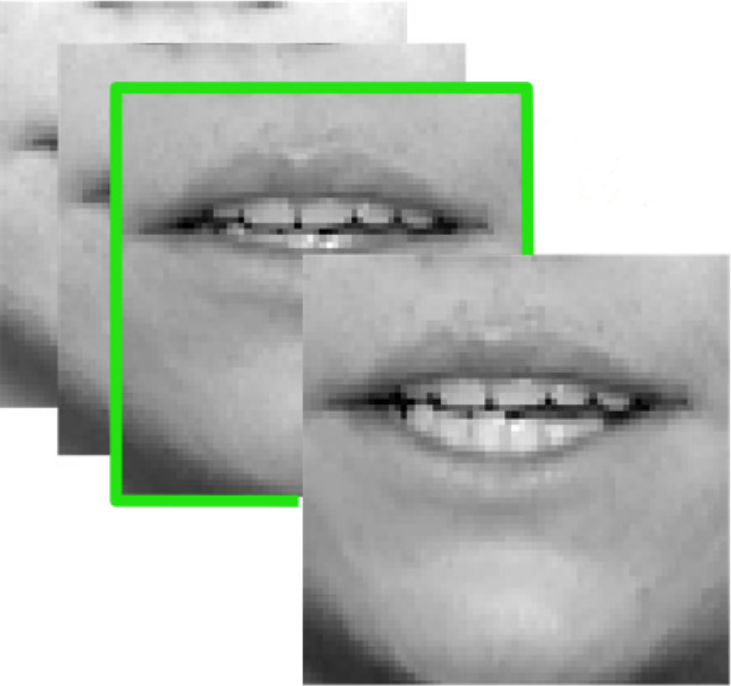
\includegraphics[width=.1\textwidth]{tikz/lips}};

  % mu, sigma, sample boxes
  \node [label={above:$\bs{\mu}^{av}_{\bs{\mylz}}(\bs{\myos}_n,\bs{\myov}_n)$}, fit=(mu-1) (mu-3), draw] (mu) {};
  \node [label={below:$\bs{\sigma}^{av}_{\bs{\mylz}}(\bs{\myos}_n,\bs{\myov}_n)$}, fit=(sigma-1) (sigma-3), draw] (sigma) {};
  \node [fit=(sample-1) (sample-3), draw] (sample) {};

  % mu, sigma, sample connections
  \draw[dashed] (mu.east) edge (sample.west) (sigma.east) -- (sample.west);
  \foreach \a in {1,2,3}
  \foreach \b in {1,2,3} {
      \draw[-] (encoder-2-\a) -- (mu-\b);
      \draw[-] (encoder-2-\a) -- (sigma-\b);
      \draw[-] (sample-\a) -- (decoder-1-\b);
      \draw[-] (cond-\a) -- (decoder-1-\b);
    }

  % input + output labels
%   \foreach \idx in {1,...,4} {
%       \node[left=0 of encoder-1-\idx] {$x_\idx$};
%       \node[right=0 of decoder-2-\idx] {$\hat x_\idx$};
%     }
  \node[above=0.1 of encoder-1-1] {$\bs{\myos}_n$};
  \node[below=0.1 of encoder-1-6] {$\bs{\myov}_n$};
  \node[above=0.1 of decoder-2-1] {$\hat{\bs{\myos}}_n$};

\end{tikzpicture}
